
\begin{sectionblock}{A Broader Focus}
  CuratedCourses was originally demonstrated with linear algebra,
  seeing as it is a topic which can be taught from many perspectives.
  The CuratedCourses team now proposes scaling-up to other courses.
\end{sectionblock}

\begin{sectionblock}{The Platform}
%  \begin{columns}
%    \begin{column}{0.5\textwidth}
%      The project team developed a platform for hosting and disseminating
%%      open mathematics content.
%    \end{column}
%    \begin{column}{0.5\textwidth}
%        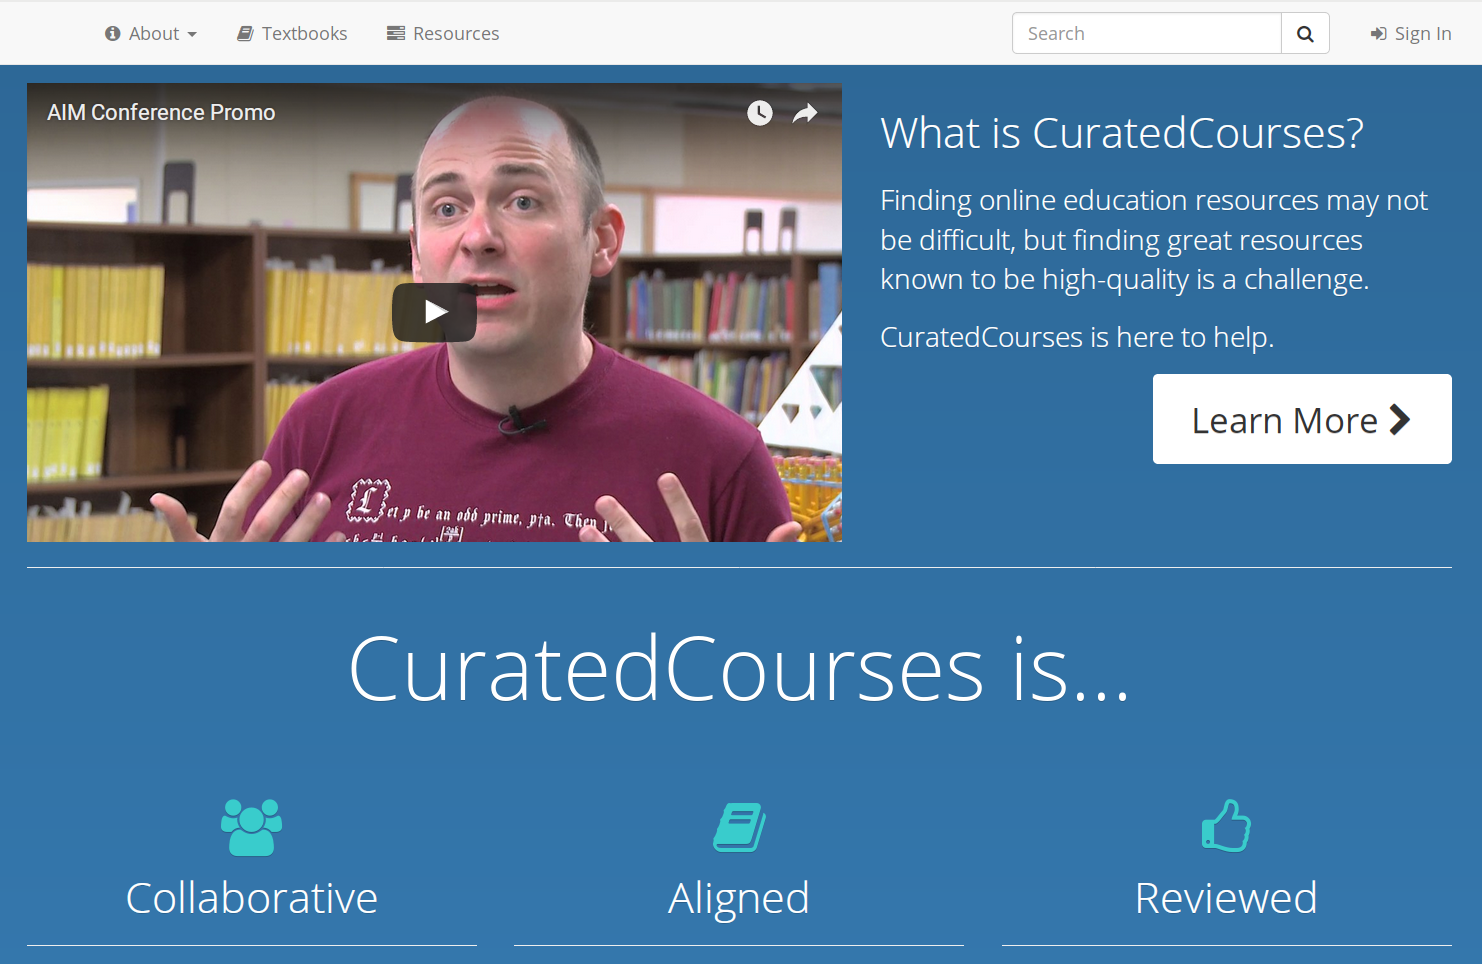
\includegraphics[width=\textwidth]{landing-page.png}
%    \end{column}
%  \end{columns}

  \begin{wrapfigure}{R}{0.40\textwidth}
    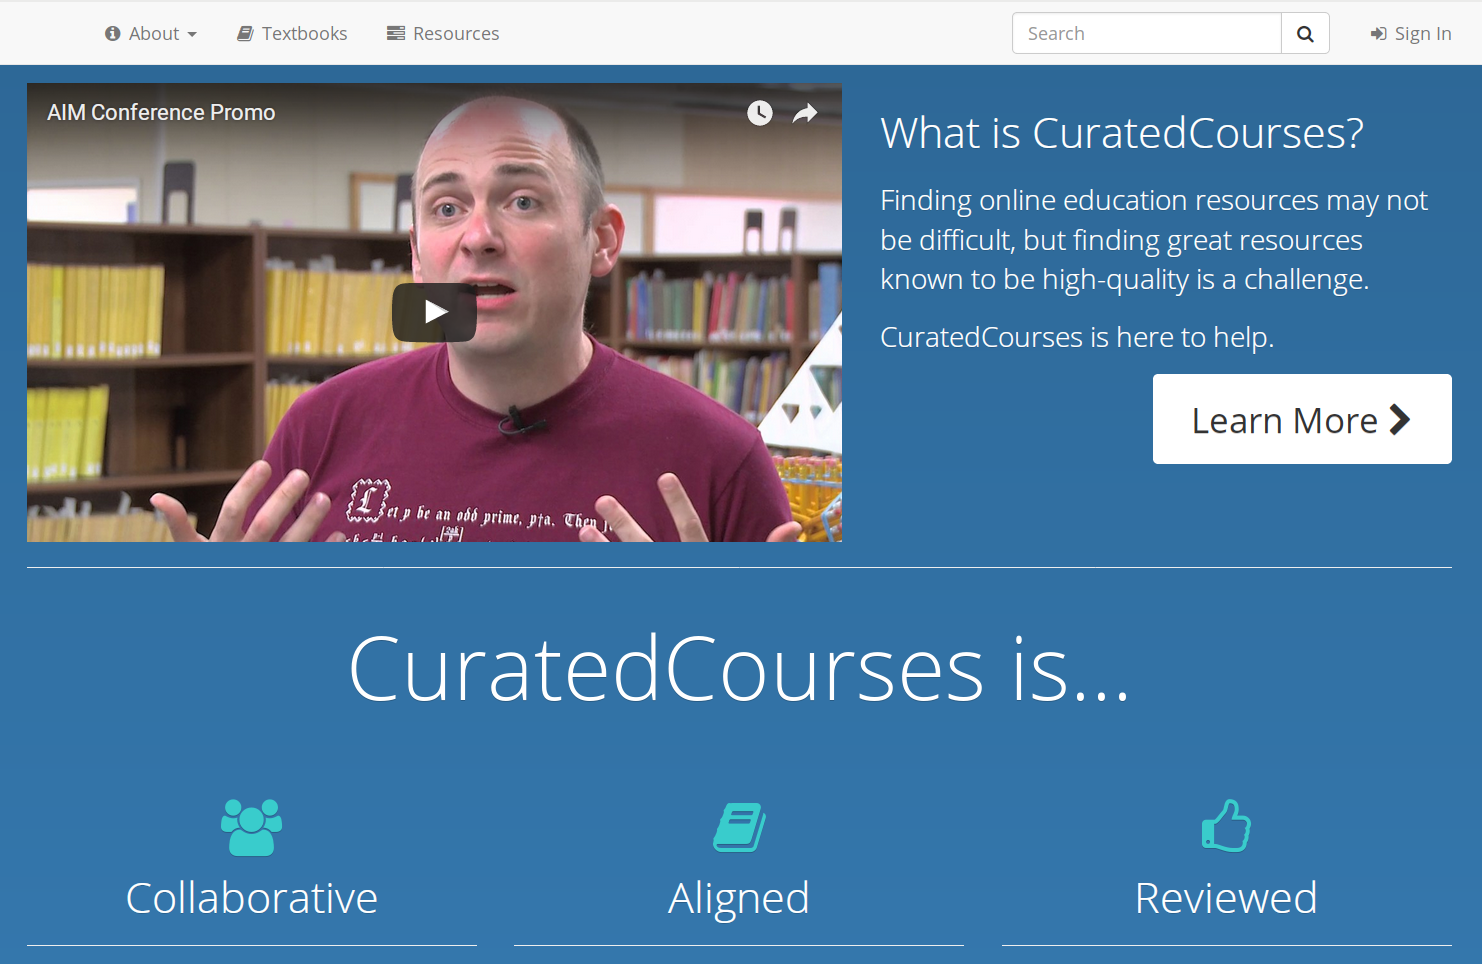
\includegraphics[width=0.38\textwidth]{landing-page.png}
  \end{wrapfigure}

  The CuratedCourses website organizes and hosts open mathematics content.  A resource submitted to the
  platform enters a moderation queue, permitting curation by experts.
\end{sectionblock}
  
  \begin{sectionblock}{Taxonomies}
  
    A fine-grained taxonomy of
   topics and learning outcomes
  permit the alignment of high-quality resources to popular textbooks.

    \begin{figure}
      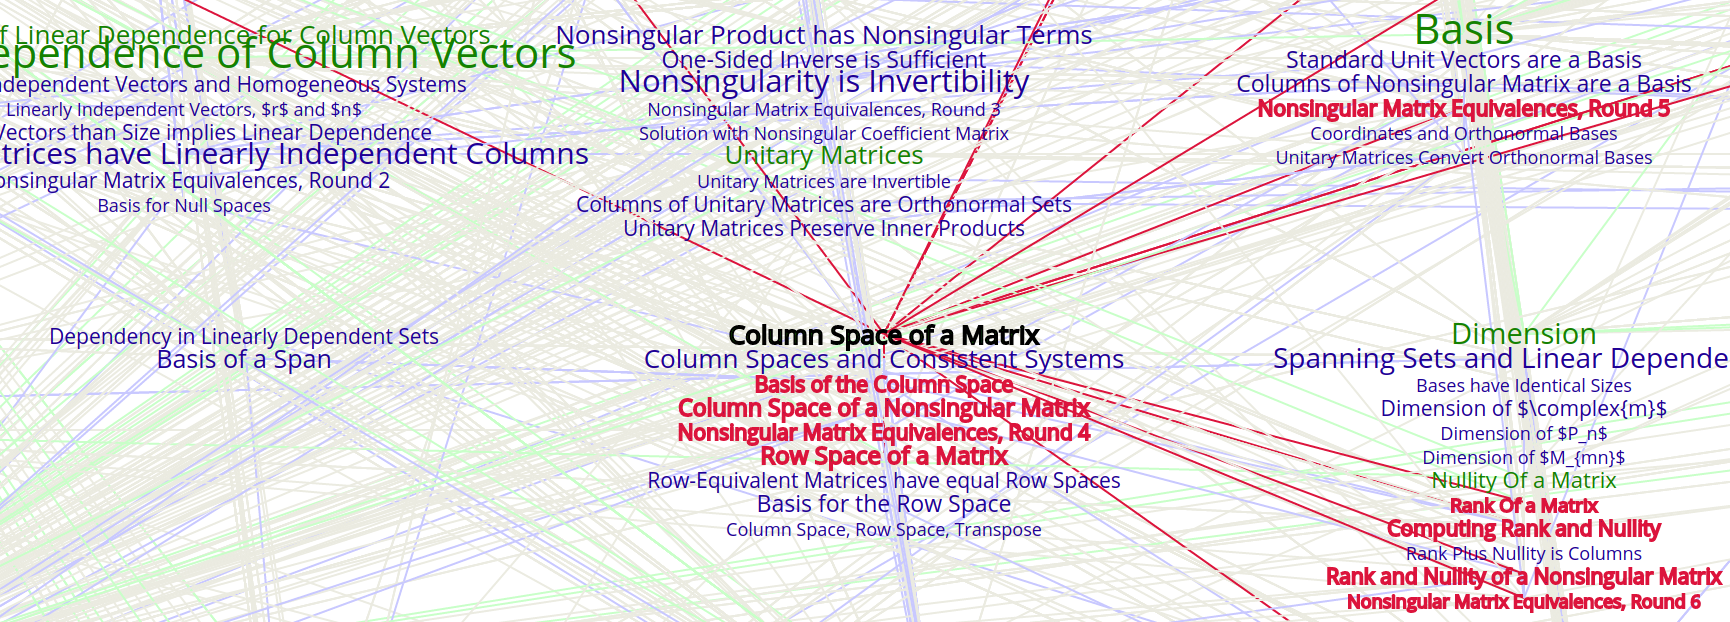
\includegraphics[width=0.65\textwidth]{topics.png}
    \end{figure}
  
\end{sectionblock}


    
